\documentclass[UTF8]{ctexart}
\CTEXsetup[format={\Large\bfseries}]{section}%默认一级标题居左
\usepackage{geometry}
\geometry{left=2.5cm,right=2.5cm,top=2.5cm,bottom=2.5cm} %页边距
\usepackage{graphicx}%图形
\usepackage{fancyhdr}%页眉页脚
\pagestyle{fancy}	%启用fancy风格设置
\lhead{}
\chead{}
\rhead{\bfseries\textsl{\today}  } % textsl 斜体
\lfoot{}
\cfoot{\thepage}
\rfoot{}
%\renewcommand{\headrulewidth}{0.6pt}    %单线页眉的设置 
\renewcommand{\footrulewidth}{0.4pt}     %单线页脚的设置 
%-----------双线页眉的设置  
\makeatletter % 进入“内部命令模式”(允许使用 @ 符号的 LaTeX 内部变量)
\def\headrule{{\if@fancyplain\let\headrulewidth\plainheadrulewidth\fi%
		\hrule\@height 1.0pt \@width\headwidth\vskip1pt%上面线为1pt粗  
		\hrule\@height 0.5pt\@width\headwidth  %下面0.5pt粗            
		\vskip-2\headrulewidth\vskip-4pt}      %两条线的距离1pt        
		  \vspace{3mm}}     %双线与下面正文之间的垂直间距 
\makeatother    % 退出“内部命令模式”
%------------双线页眉的设置            
% \usepackage{booktabs}
% \usepackage{subfigure}
\usepackage{setspace}
\usepackage{amsmath}
\usepackage{array}%需要该宏包
\usepackage{diagbox} % 加载宏包
\usepackage{multirow}
\usepackage{textcomp}
\usepackage{indentfirst}%首行缩进宏包
\usepackage{setspace}
\usepackage{amssymb}
\usepackage{listings}
\usepackage{xcolor}    % 可选:代码着色(示例用)
\lstset{
    frame = single,                % 添加边框(single 表示单线边框)
    numbers = left,                % 在左侧显示行号
    numberstyle = \tiny\color{gray}, % 行号样式
    basicstyle = \ttfamily,        % 设置等宽字体
    keywordstyle = \color{blue},    % 关键字颜色
    commentstyle = \color{green},   % 注释颜色
    stringstyle = \color{red},      % 字符串颜色
    breaklines = true,             % 自动换行
    showstringspaces = false,      % 不显示字符串中的空格
    tabsize = 4                    % 设置缩进空格数
}
\usepackage[colorlinks=true,pdfborder={0 0 0},
    linkcolor=red,     % 内部链接(如目录→章节)的文字颜色
    citecolor=green,    % 引用(如\cite)的文字颜色
    urlcolor=blue,      % 网址的文字颜色
]{hyperref} %超链接
\usepackage{float}  % 提供 [H] 选项

\title{{\heiti  第三周实验:命令行环境、python基础、py图形库 }\vspace{-2em}}
\date{}
\begin{document}
\thispagestyle{empty}  %用于设置 “当前页” 的页眉页脚风格:
\begin{figure}[tph!] %封面标题
	\centering
	
\includegraphics[width=0.7\linewidth]{figure/2}
	
\end{figure}

\begin{center}% % 内容居中环境(所有内部内容均居中对齐)
	\quad \\ %插入一个小空格
	\quad \\
	\quad \\
	\quad \\
	% \quad \\
	% \quad \\
	\heiti \fontsize{30}{17} \quad \quad 第\quad 三\quad 周\quad \quad \quad 
	\vskip 0.5cm
	\songti \zihao{2} 实\quad 验\quad 报\quad 告%在此打印论文题目,二号黑体	
\end{center}
\vskip 1cm

\begin{quotation}
	\songti \fontsize{20}{20}
	\doublespacing
	\par\setlength\parindent{12em}
	\qquad
\begin{center}
		{\Large 学\hspace{0.88cm} 院:\underline{\hbox to 58mm{信息科学与工程学部\hfill}}}
		\vskip 0.3cm	
		{\Large 班\hspace{0.88cm} 号:\underline{\hbox to 58mm{计科一班\hfill}}}
		\vskip 0.3cm
		{\Large 姓\hspace{0.88cm} 名:\underline{\hbox to 58mm{顾晓宁\hfill}}}
		\vskip 0.3cm	
		{\Large 学\hspace{0.88cm} 号:\underline{\hbox to 58mm{24020007036\hfill}}}
		\vskip 0.3cm	
		{\Large 实验编号:\underline{\hbox to 58mm{第三周实验报告\hfill}}}
		\vskip 0.3cm	
		{\Large 指导教师:\underline{\hbox to 58mm{周小伟\hfill}}}
	\end{center}
	% \vskip 3cm
	% \begin{flushright}% 日期右对齐
	% 	% 2019\;年\;5\;月\;14\;日
	% 	\today
	% \end{flushright}
	
\end{quotation}
\newpage
%\thispagestyle{empty}
\tableofcontents % 自动生成目录(基于后续的 \section、\subsection 等章节命令)
\newpage
\maketitle	
\thispagestyle{fancy}	
\section{实验目的}
\textbf{学习配置基本的命令行环境,学习如何使用ssh连接服务器,以及python基础及其图形库}

\section{练习内容与结果}
\subsection{Python基础}
\href{file:py-basic-review.txt}{查看文件}\\
\indent \hbox{因为具有一定的py基础,部分内容不附上,可参见参考资料页的连接。}
\\
\indent \href{file:py-basic-test/main.py}{这是一部分练习用例,有关list}

\subsubsection{list:创建、访问、修改}
\begin{verbatim}
	创建:
	list()
	var = [e[,e...]]
	等
	访问:
	使用[]下标索引可访问元素,支持负数索引
	可以使用切片[start:end:step]
	修改略
\end{verbatim}

\subsubsection{list:+ * list()}
\begin{verbatim}
	+ 拼接
	* 重复,注意浅拷贝等问题
	list() 转化为list
\end{verbatim}

\subsubsection{list:函数若干}
\begin{verbatim}
	1	len(list)
	列表元素个数
	2	max(list)
	返回列表元素最大值
	3	min(list)
	返回列表元素最小值
	4	list(seq)
	Python包含以下方法:
\end{verbatim}

\subsubsection{list:方法若干}
\begin{verbatim}
	1	list.append(obj)
	在列表末尾添加新的对象
	2	list.count(obj)
	统计某个元素在列表中出现的次数
	3	list.extend(seq)
	在列表末尾一次性追加另一个序列中的多个值(用新列表扩展原来的列表)
	4	list.index(obj)
	从列表中找出某个值第一个匹配项的索引位置
	5	list.insert(index, obj)
	将对象插入列表
	6	list.pop([index=-1])
	移除列表中的一个元素(默认最后一个元素),并且返回该元素的值
	7	list.remove(obj)
	移除列表中某个值的第一个匹配项
	8	list.reverse()
	反向列表中元素
	9	list.sort(cmp=None, key=None, reverse=False)
	对原列表进行排序
\end{verbatim}


\subsection{py图形库基础}
\href{file:py-graphy.txt}{基础语法}
\\
\indent 以下涉及的Pillow库的基本演示,可以见该目录下的py-code-test文件夹,内附有demo。
\\
\indent	\href{file:py-code-test/main.py}{代码文件}
\subsubsection{Pillow库:打开、访问、展示、保存?}
\begin{verbatim}
	1. 打开和创建图像
	打开现有图像,参数是路径:
	使用 Image.open() 函数。
	创建新图像:
	使用 Image.new() 函数。
	# 例如
	new_img = Image.new('RGB', (400, 300), color='red')

	2. 图像的基本属性
	即类Image的属性
	format      # 图像格式 (e.g., JPEG, PNG)
	size        # 图像尺寸 (宽度, 高度)
	width       # 图像宽度
	height      # 图像高度
	mode        # 颜色模式 (e.g., RGB, RGBA, L (灰度), CMYK)

	3. 显示图像
	img.show()  # 会使用系统默认的图片查看器打开图像
	
	4. 保存图像
	使用 save() 方法,可以指定格式和质量等参数。
	img.save('new_image.png')           # 根据扩展名自动判断格式
	img.save('output.jpg', 'JPEG')      # 明确指定格式
	img.save('high_quality.jpg', quality=95)  # 保存为高质量JPEG (1-100, 默认75)
	img.save('small_size.png', optimize=True) # 优化PNG文件大小
\end{verbatim}

\subsubsection{Pillow库: 转换图像模式}
\begin{verbatim}
	使用方法convert
	gray_img = img.convert('L')    # 转换为灰度图像
	rgba_img = img.convert('RGBA') # 转换为带透明通道的图像
\end{verbatim}

\subsubsection{Pillow库:调整图像大小}
\begin{verbatim}
	1.resize() 方法:
	# 缩放到指定尺寸
	resized_img = img.resize((400, 300))

	# 高质量缩放推荐使用 Lanczos 滤波器
	resized_img = img.resize((400, 300), Image.LANCZOS)

	2.thumbnail() 方法:
	原地修改,生成保持原图宽高比的缩略图
	尺寸参数是一个元组,表示最大宽度和高度。
	例如:
	img.thumbnail((150, 150)) # 图像的宽或高将被限制在150像素以内,比例不变
\end{verbatim}

\subsubsection{Pillow库:裁剪图像}
\begin{verbatim}
	使用 crop() 方法,参数是一个定义左、上、右、下像素坐标的元组 (left, upper, right, lower)。
	注意右下坐标分别大于左上,原点为图像左上角。
\end{verbatim}

\subsubsection{Pillow库:旋转和翻转}
\begin{verbatim}
	1.旋转 rotate()
	# 旋转45度,并扩展画布以避免图像被裁剪,背景填充为白色
	rotated_img = img.rotate(45, expand=True, fillcolor='white')

	2.翻转 transpose()
	# 水平翻转
	flipped_img = img.transpose(Image.FLIP_LEFT_RIGHT)
	# 垂直翻转
	flipped_img = img.transpose(Image.FLIP_TOP_BOTTOM)
\end{verbatim}

\subsubsection{Pillow库:图像粘合}
\begin{verbatim}
	使用 paste() 方法可以将一张图像粘贴到另一张图像上。
	paste() 会原地修改 img1。
	# 假设有 img1 和 img2
	# 将 img2 粘贴到 img1 的 (x, y) 坐标处
	img1.paste(img2, (50, 50))
	可以作为水印
\end{verbatim}

\subsubsection{Pillow库:图像增强}
\begin{verbatim}
	需要先导入对应模块,
	from PIL import ImageEnhance
	# 增强对比度
	enhancer = ImageEnhance.Contrast(img)
	enhanced_img = enhancer.enhance(2.0) # 增强2倍

	# 增强亮度
	enhancer = ImageEnhance.Brightness(img)
	bright_img = enhancer.enhance(1.5)   # 增强1.5倍

	# 增强色彩饱和度
	enhancer = ImageEnhance.Color(img)
	colorful_img = enhancer.enhance(1.5)

	# 增强锐度
	enhancer = ImageEnhance.Sharpness(img)
	sharp_img = enhancer.enhance(2.0)
\end{verbatim}



\subsection{命令行环境}
\href{file:cmd-line-env.txt}{文字版}
\subsubsection{如何停止作业/进程?}
一般可以使用ctrl+c 或者 ctrl+\verb|\| 或者 kill -TERM  PID,来结束一个进程,也可使用kill 作业号,来结束一个作业。\\
\indent 核心转储是指接受SIGQUIT信号/程序意外终止,将其快照存为一个文件,通常命名为core.PID,可用以调试。或调用apport自动处理崩溃报告。
\begin{figure}[H]
	\centering
	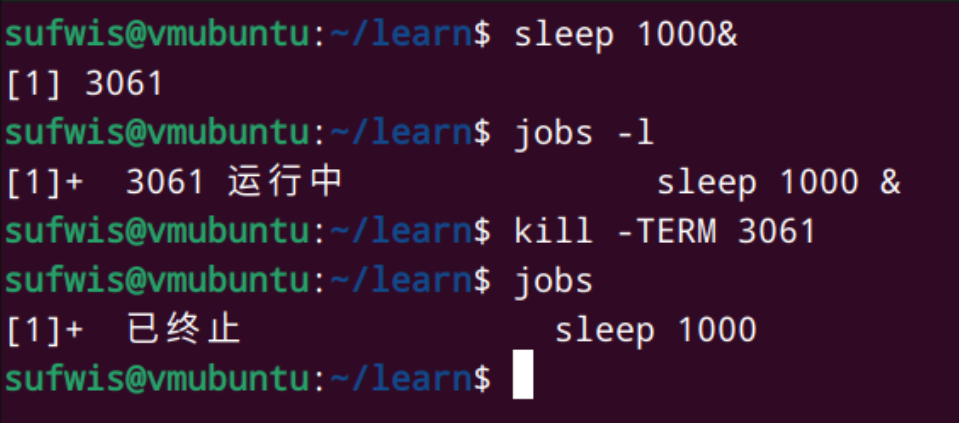
\includegraphics[width=0.7\linewidth]{figure/kill_TERM.png}
	\caption{kill -TERM 如图}
\end{figure}
\begin{figure}[H]
	\centering
	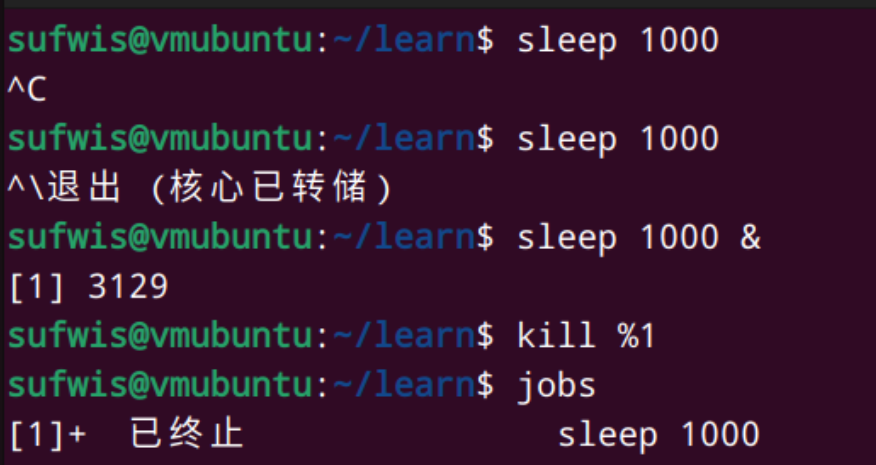
\includegraphics[width=0.7\linewidth]{figure/kill_other.png}
	\caption{其他结束方式 如图}
\end{figure}

\subsubsection{如何暂停进程,暂停后可以进行那些操作?}
ctrl+z可暂停并将之转为后台,使用jobs查看后台的作业情况,\verb|%|+作业号选取作业。之后使用fg或bg将之转为前台进行或后台进行。
\\
\indent kill -STOP 作业号,暂停;kill -CONT 作业号,继续进行;
\\
\indent 使用命令+ \verb|&|直接在后台运行,不过此时仍旧为shell子进程,shell推出后,都会结束运行。
在输入命令时使用nohup,或者使用disown分离一个作业,这样在该shell结束时,该作业不会结束。
\begin{figure}[H]
	\centering
	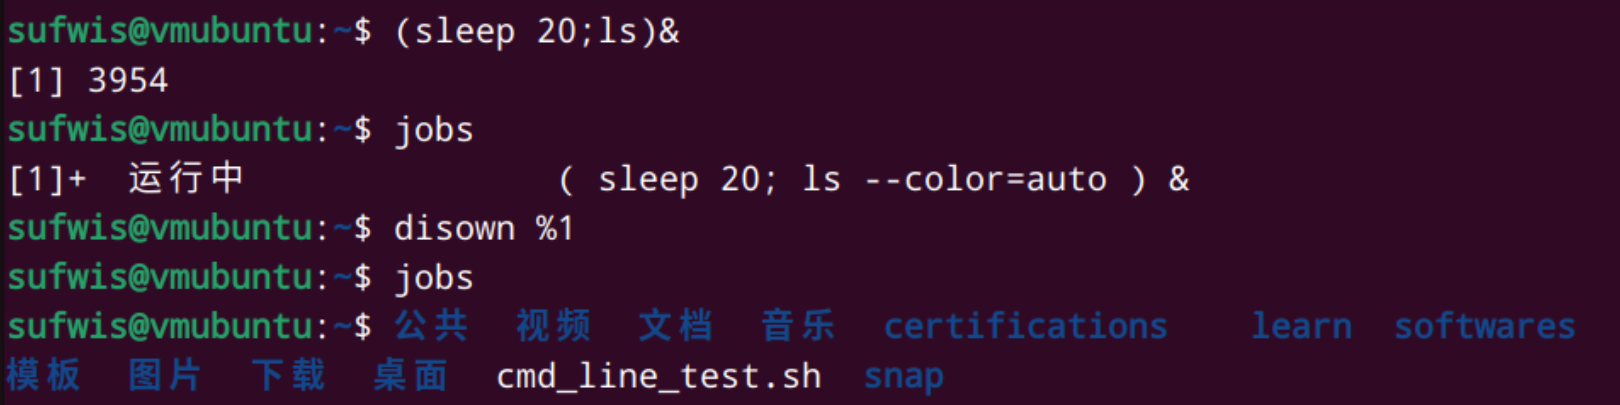
\includegraphics[width=0.7\linewidth]{figure/disown.png}
	\caption{disown将作业从当前shell中移除 如图}
\end{figure}

\subsubsection{tmux的会话的使用?}
tmux或tmux new -s name创建一个会话,tmux ls 查看会话,tmux a -t name 连接会话,
倘若已连接,<C-b>+d分离会话,返回终端,tmux -kill-session -t name 删除会话
\begin{figure}[H]
	\centering
	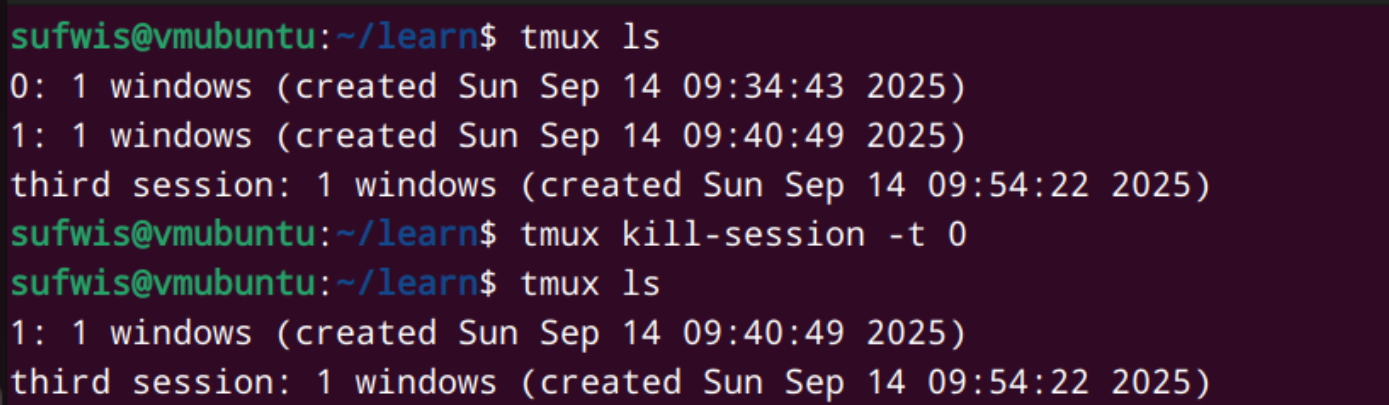
\includegraphics[width=0.7\linewidth]{figure/tmux_session.png}
	\caption{删除会话 如图}
\end{figure}

\subsubsection{tmux的窗口使用?}
\begin{verbatim}
	<C-b> c 创建一个新的窗口,使用 <C-d> 关闭
	<C-b> N 跳转到第 N 个窗口,注意每个窗口都是有编号的
	<C-b> p 切换到前一个窗口
	<C-b> n 切换到下一个窗口
	<C-b> , 重命名当前窗口
	<C-b> w 列出当前所有窗口
\end{verbatim}
\begin{figure}[H]
	\centering
	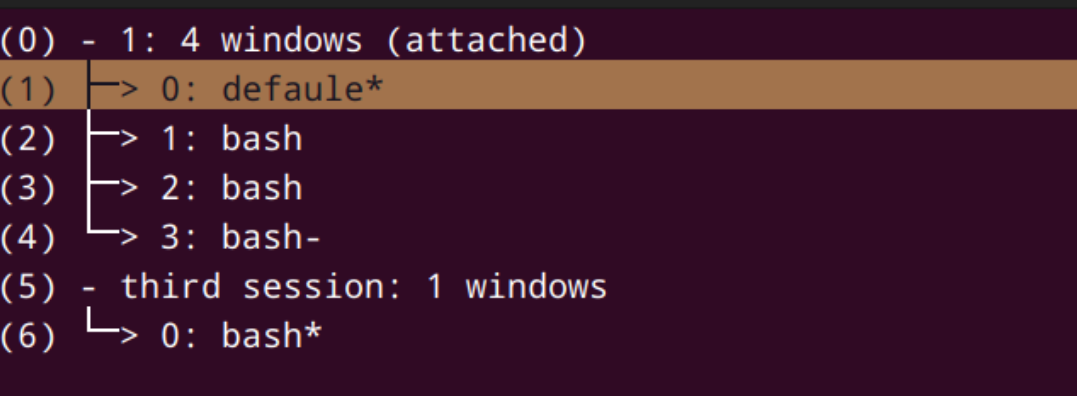
\includegraphics[width=0.7\linewidth]{figure/tmux_windows.png}
	\caption{列出当前所有窗口 如图}
\end{figure}

\subsubsection{tmux的面板使用?}
\begin{verbatim}
	面板是 tmux 中最小的工作区域,每个面板都可以独立运行一个进程,一个伪终端
	<C-b> " 水平分割
	<C-b> % 垂直分割
	<C-b> <方向> 切换到指定方向的面板,<方向> 指的是键盘上的方向键
	<C-b> z 切换当前面板的缩放
\end{verbatim}
\begin{figure}[H]
	\centering
	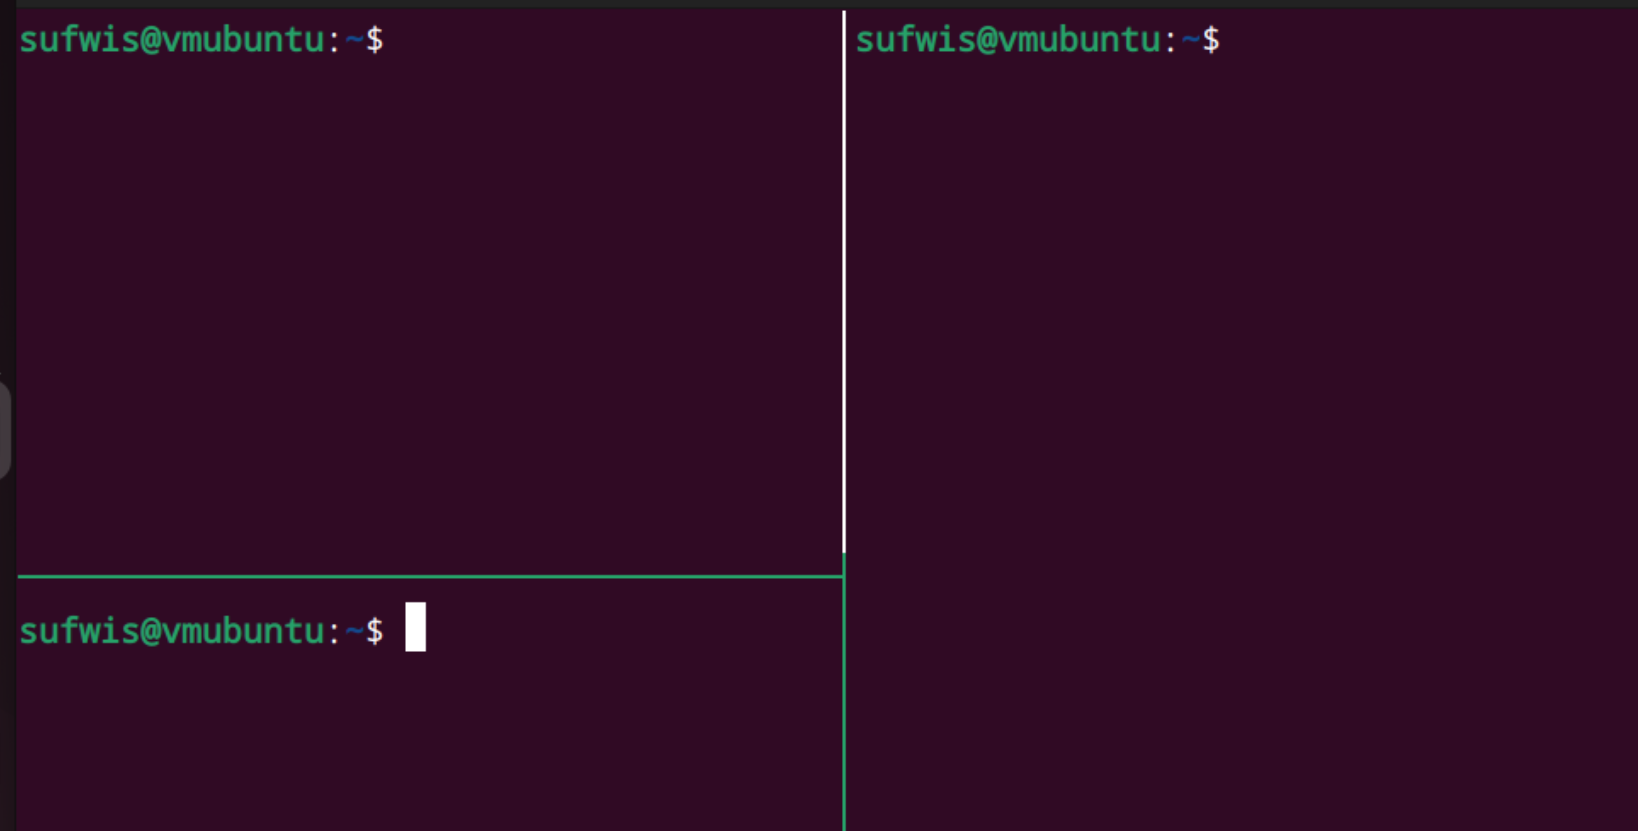
\includegraphics[width=0.7\linewidth]{figure/tmux_panel.png}
	\caption{使用垂直分割和水平分割 如图}
\end{figure}

\subsubsection{别名alias的使用与配置?}
\begin{verbatim}
	alias alias_name="command_to_alias arg1 arg2"
\end{verbatim}
\indent 即可设定临时别名,如果放入.bashrc或对应的配置文件中,可以永久使用。
\begin{figure}[H]
	\centering
	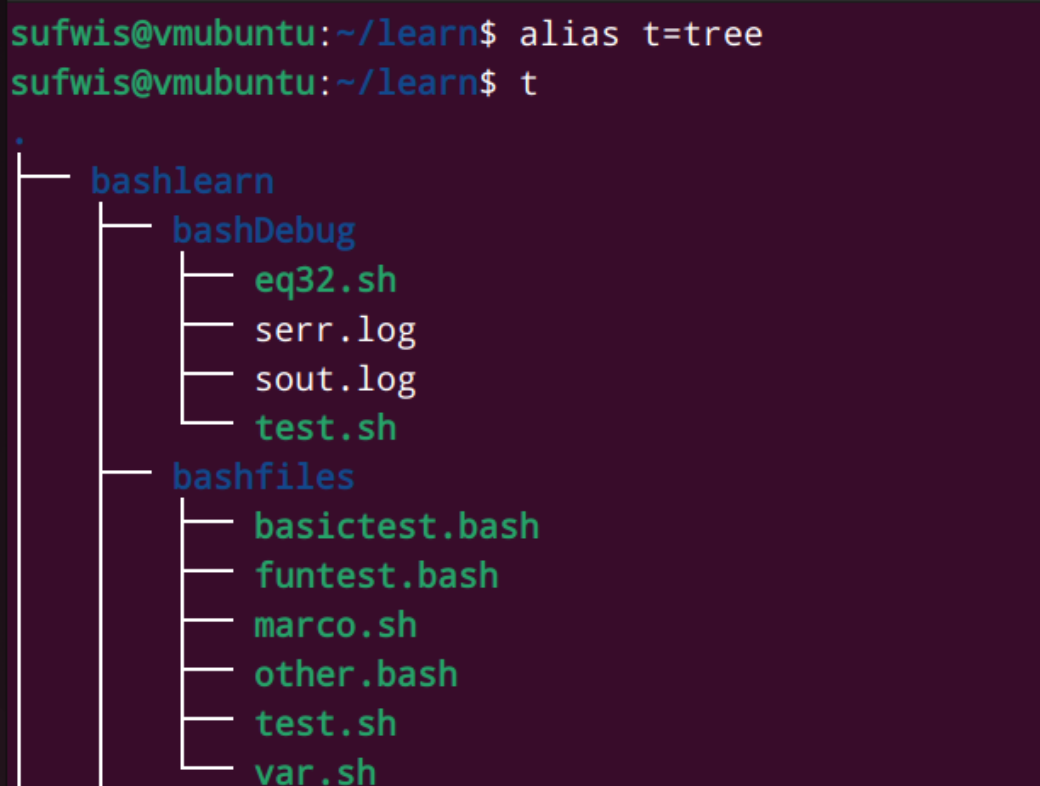
\includegraphics[width=0.7\linewidth]{figure/alias.png}
	\caption{临时别名 如图}
\end{figure}
\indent 假设使用tmux开启另一个shell进程,显示无该命令。
\begin{figure}[H]
	\centering
	
\includegraphics[width=0.7\linewidth]{figure/tmux_alias_temp.png}
	\caption{如图}
\end{figure}
\indent 在.bashrc中加入别名配置,然后在另一个终端中使用。
\begin{figure}[H]
	\centering
	
\includegraphics[width=0.7\linewidth]{figure/bashrc.png}
	\caption{配置 如图}
\end{figure}
\begin{figure}[H]
	\centering
	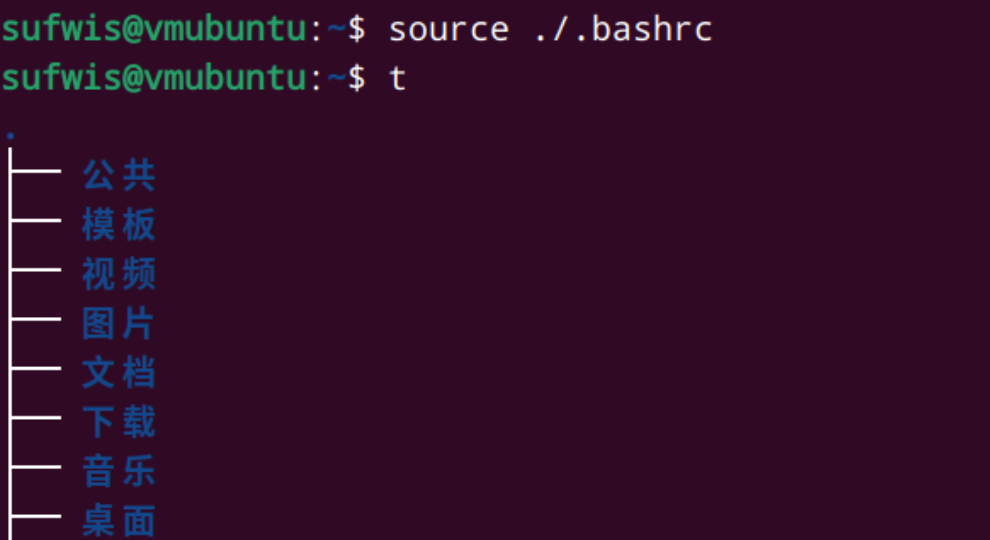
\includegraphics[width=0.7\linewidth]{figure/tmux_alias.png}
	\caption{使用 如图}
\end{figure}

\subsubsection{ssh安装与使用?}
\begin{lstlisting}
	# linux server
	sudo apt install openssh-server # load
	sudo systemctl start ssh # start ssh-server
	sudo systemctl enable ssh # Set as self starting upon startup
	sudo systemctl status ssh # check whether is started

	# client
	ssh username@host # then enter pwd
\end{lstlisting}

\subsubsection{ssh密钥?}
\begin{lstlisting}
	ssh-keygen
	ssh-copy-id -i ~/.ssh/id_rsa.pub ubuntu@192.168.1.105
\end{lstlisting}
\begin{verbatim}
	之后默认生成在~/.ssh/id_rsa,或用户名/.ssh/id_rsa(Windows)。
	id_rsa为私钥,id_rsa.pub:公钥(可公开,用于配置到远程服务器),
	将公钥拷贝到你要连接的服务器的.ssh/authorized_keys 内,即可无需密码登录。
\end{verbatim}
\qquad 如果未使用默认路径,可在对应命令处使用-i指明密钥的路径。
\\
\indent 如果无法使用ssh-copy-id可以手动复制。
\begin{figure}[H]
	\centering
	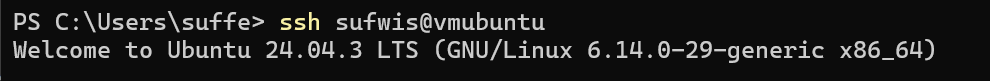
\includegraphics[width=0.7\linewidth]{figure/ssh.png}
	\caption{密钥无密码登录 如图}
\end{figure}

\subsubsection{scp复制文件?}
\begin{verbatim}
	scp [本地文件路径] [远程用户]@[远程IP或域名]:[远程目标路径]
	scp [远程用户]@[远程IP或域名]:[远程文件路径] [本地目标路径]
	SCP命令总是在源文件所在的那一端执行
	SCP命令的执行位置决定了它能访问的文件系统,SCP命令总是在包含源文件的那一端执行
\end{verbatim}
\begin{figure}[H]
	\centering
	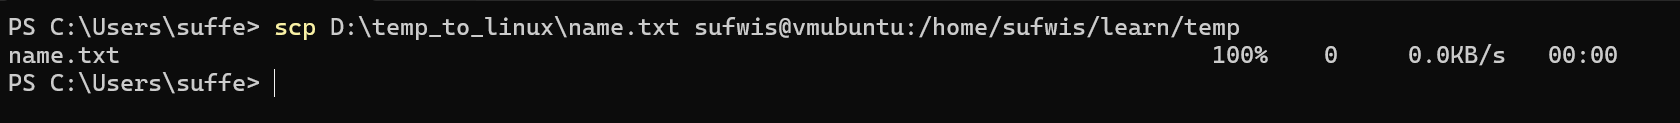
\includegraphics[width=0.7\linewidth]{figure/win_to_linux.png}
	\caption{win文件转Linux虚拟机 如图}
\end{figure}
\begin{figure}[H]
	\centering
	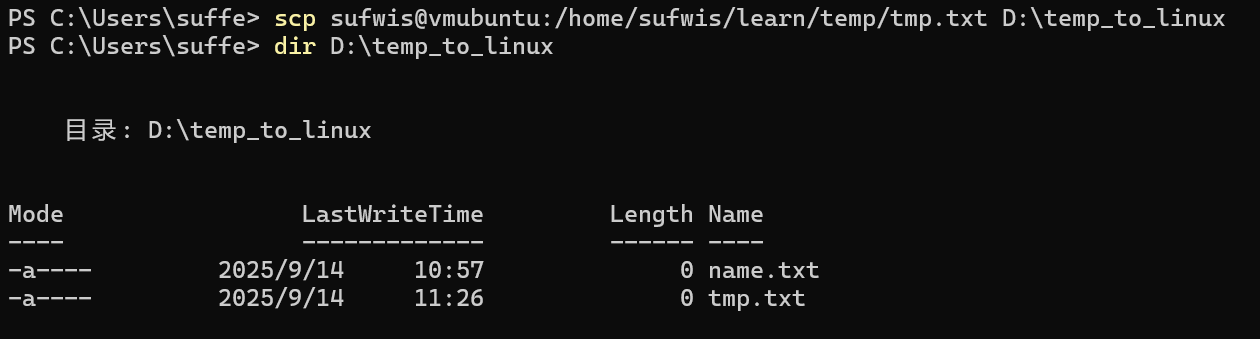
\includegraphics[width=0.7\linewidth]{figure/linux_to_win.png}
	\caption{Linux虚拟机文件转win 如图}
\end{figure}


\section{实验感悟}
python越来越流行,学习人数也越来越多。相对而言,python的语法简单,虽然运行效率相对低,但是相应的开发效率却很高。
这离不开python多样的库、模块等。
\\
\indent ssh的使用同样普遍,例如连接云服务器。总之学无止境。

\section{个人github/gitee账号}
\href{https://github.com/sufwis/development-tools-learn.git}{对应仓库}
\\
\indent \href{https://github.com/sufwis}{个人github账号}

\section{友情链接}
\href{https://missing-semester-cn.github.io/2020/command-line/}{命令行环境}
\\
\indent \href{https://www.runoob.com/python/python-tutorial.html}{Python 基础教程}
\\
\indent \href{https://blog.csdn.net/sgzqc/article/details/124871774}{【Python】推荐五个常用的图像处理库}


\end{document}